\documentclass{article}
\usepackage{graphicx} % Required for inserting images
\graphicspath{ {./images/} }
\usepackage{diagbox}
\usepackage{amsmath}
\usepackage{amsfonts}

\title{MA677-Final Project}
\author{Ajay Krishnakumar }
\date{May 2024}

\begin{document}

\maketitle{}

\textbf{Notes on Chapter 5: Uncertainty Due to Ignorance of State of Nature from Elements of Decision Theory by Chernoff and Moses}



\section{Chapter Overview}

The goal of the chapter is to use utility to quantify what strategies (denoted by s) to take based on observations(denoted by x's) about unknown states and the set of actions available. It starts off discussing how to break these down into the expected losses for each state of nature, $\theta$, plot them and figure out where the mixed strategies lie using the concept of convex sets. These concepts are slowly built upon to talk about dominated strategies and eventually, choosing an optimum strategy - using Bayes Strategies and minmax. The chapter then turns to addressing this in higher dimensions. 

Mathematically, I'll focus on the optimization in higher dimensions, just because I find it interesting. I'll use programming to create illustrations of surfaces in three dimensions to illustrate the same things the chapter covers in two dimensions. 

The long and short of this is, I'll use a three dimensional case instead of a two dimensional one to follow the reasoning of the chapter and hopefully be a little more deliberate in extending the talk of higher dimensions to general cases. 

\section{Taking the Chapter's overarching example to the next dimension}
Mr. Nelson is visiting the blustery(or not) isle of North Phiggins. He needs to decide what to wear(his actions) based on what a weather indicator(the observations) say about the conditions on each day (the state of nature). I'll extend the two states of nature in the example to three here - this provides a way to work through the chapter without repeating exactly what the chapter does and as a launching point for looking into the strategies outlined in the chapter in higher dimensions.

Let the set of actions Mr. Nelson can take be $a_1$: Shorts and a t shirt, $a_2$: Shorts and a t shirt, but with a raincoat, $a_3$: Trousers instead of shorts, raincoat, hat, wellies. Essentially, Mr.Nelson can wear a fair weather outfit, a foul weather outfit and a very foul weather outfit.  

The weather indicator also takes on three values: fair, foul, very foul. This gives us 27 possible pure strategies Mr.Nelson can take - three possible actions for each weather reading. Obviously some of these strategies are nonsensical such as wearing shorts and a t shirt regardless of what you expect the weather to be (although, as I say that, a quick survey of any college campus in the depths of winter will prove that such people do in fact exist), but we'll come back to that when we talk about dominated strategies. 

The loss of utility table given each action and state of nature is as follows:

\begin{table}[htb]
\begin{center}
    
\begin{tabular}{|l|c|c|c|}\hline
\diagbox[width=5em]{\\$\theta$}{\\a}&
  $a_1$ & $a_2$ & $a_3$ \\ \hline
  $\theta_1$ & 0 & 1 & 7 \\ \hline
  $\theta_2$ & 4 & 3 & 4 \\ \hline
  $\theta_3$ & 9 & 5 & 2 \\ \hline
\end{tabular}
\end{center}
\caption{Loss of utility for each action and state of nature}
\end{table}



The probability of observing a reading on the weather device, given a certain state of nature $\theta$ is given by the following table:

\begin{table}[htb]
\begin{center}
    
\begin{tabular}{|l|c|c|c|}\hline
\diagbox[width=5em]{\\$\theta$}{\\a}&
  $x_1$ & $x_2$ & $x_3$ \\ \hline
  $\theta_1$ & 0.60 & 0.25 & 0.15 \\ \hline
  $\theta_2$ & 0.20 & 0.30 & 0.50 \\ \hline
  $\theta_3$ & 0.05 & 0.27 & 0.68 \\ \hline
\end{tabular}
\end{center}
\caption{$\mathbb{P}(\textbf{X}=x|\theta)$}
\end{table}


For each of the 27 possible strategies, we can use the tables above to calculate expected loss. The code to reproduce this is in the rmd file titled 'StrategiesCalculated' on the github. 

The table of expected losses for strategies is laid out below.


    
\begin{tabular}{|l|c|c|c|c|c|c|c|c|}\hline
\diagbox[width=15em]{State of Nature\\$\theta$}{Strategy, s \\a}&
  $s_1$ & $s_2$ & $s_3$ & $s_4$ & $s_5$ & $s_6$ & $s_7$ & $s_8$   \\ \hline
  $\theta_1$ & 0 & 0.15 & 1.05 &0.25 & 0.40 & 1.30 & 1.75 & 1.90  \\ \hline
  $\theta_2$ & 4.00 & 3.50 & 4.00 & 3.70 & 3.20 & 3.70 & 4.00 & 3.50  \\ \hline
  $\theta_3$ & 9.00 &6.28 & 4.24 & 7.92 & 5.20 & 3.16 & 7.11 & 4.39  \\ \hline
\end{tabular}
\hfill

\begin{tabular}{|l|c|c|c|c|c|c|c|c|}\hline
\diagbox[width=15em]{State of Nature\\$\theta$}{Strategy, s \\a}&
  $s_9$ & $s_{10}$ & $s_{11}$ & $s_{12}$ & $s_{13}$ & $s_{14}$ & $s_{15}$ & $s_{16}$   \\ \hline
  $\theta_1$ & 2.80 & 0.60 & 0.75 & 1.65 & 0.85 & 1.00 & 1.90 & 2.35  \\ \hline
  $\theta_2$ & 4.00 & 3.80 & 3.30 & 3.80 & 3.50 & 3.00 & 3.50 & 3.80  \\ \hline
  $\theta_3$ & 2.35 &8.80 & 6.08 & 4.04 & 7.72 & 5.00 & 2.96 & 6.91  \\ \hline
\end{tabular}

\begin{tabular}{|l|c|c|c|c|c|c|c|c|}\hline
\diagbox[width=15em]{State of Nature\\$\theta$}{Strategy, s \\a}&
  $s_{17}$ & $s_{18}$ & $s_{19}$ & $s_{20}$ & $s_{21}$ & $s_{22}$ & $s_{23}$ & $s_{24}$   \\ \hline
  $\theta_1$ & 2.50 & 3.40 & 4.20 & 4.35 & 5.25 & 4.45 & 4.60 & 5.50  \\ \hline
  $\theta_2$ & 3.30 & 3.80 & 4.00 & 3.70 & 4.00 & 3.70 & 3.20 & 3.70  \\ \hline
  $\theta_3$ & 4.19 &2.15 & 8.65 & 5.93 & 3.89 & 7.57 & 4.85 & 2.81  \\ \hline
\end{tabular}

\begin{tabular}{|l|c|c|c|}\hline
\diagbox[width=15em]{State of Nature\\$\theta$}{Strategy, s \\a}&
  $s_{25}$ & $s_{26}$ & $s_{27}$\\ \hline
  $\theta_1$ & 5.95 & 6.10 & 7.00\\ \hline
  $\theta_2$ & 3.70 & 4.00 & 3.50\\ \hline
  $\theta_3$ & 2.81 &6.76 & 4.04\\ \hline
\end{tabular}

\vspace{10mm} %5mm vertical space
Every mixed strategy between any two points can be represented as a line segment between them, between three points by the portion of a plane formed between them and between four or more points by the polyhedron formed by them. This is consistent with the definition of a convex set. I.e: For any two points in our set of strategies, the points on the line segment connecting those points is also in the set. The set of all strategies formed by the points in the table above is a polyhedron with those points as its vertices. This is the set of all mixed and pure strategies. 
\vspace{5mm} %5mm vertical space

Here's a plot of the shape, the pink, craggy, mountain looking thing is a polyhedron formed by the pure strategies of Mr. Nelson. Imagine, to borrow the textbooks wonderful analogy, popping an elastic wrapper over this shape. That wrapper defines the convex set of all mixed and pure strategies for Mr. Nelson.(If you have a look at the 3D Plots jupyter notebook file, you can play around and move this plot to get a better, less static idea of what it looks like).

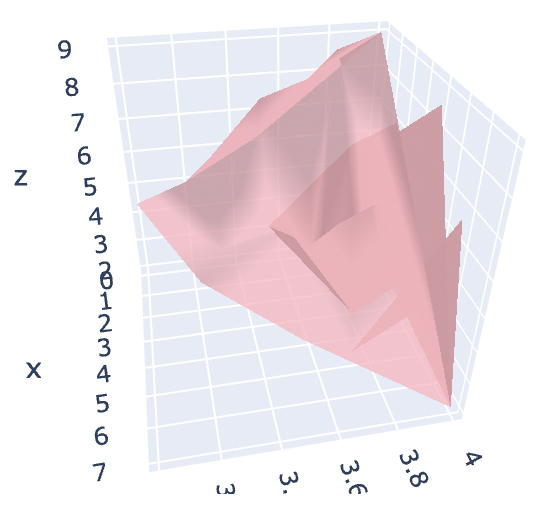
\includegraphics{images/strat_plot.png}

\vspace{5mm} %5mm vertical space
Now comes the decision theory part of this exercise. Given all these strategies, how does Mr.Nelson decide what to do? There are two approaches here that we will consider. They Bayes Strategy and Minmax solutions. Before we jump into that, a brief discussion of admissible strategy. 

A strategy is admissible if it is not dominated. A strategy is dominated if another strategy has a lower loss for all of the three states of nature we are interested in. 

We can extend Exercise 5.16 to three dimensions to prove that if two strategies are admissible, their mixed strategies are also admissible. Consider a strategy s. If we set s as the origin and divide our space into 8 'octants' we can establish that any admissible strategy that leaves s also admissible cannot be in any of two regions. The region defined by the positive direction of all three axes cannot contain a second strategy s' because s' would be dominated by s. Similarly, the region defined by the negative direction of all three axes cannot contain s' because then s' would dominate s. This means that any line connecting s and s' must also lie in the admissible regions and must therefore be admissible in and of itself. 

What does this mean for our Mr. Nelson? Well, it means that the majority of his strategies are inadmissible and the lower surface of the polyhedron defining the convex set of his strategies is the set of his admissible strategies. 

This is hard to visualize on the figure above, so consider if the convex set of his strategies is a sphere, for simplicity. Then the set of his admissible strategies is the surface defined by the bottom left quarter of the sphere. Playing around with the sphere in the 3D plots notebook should demonstrate this. But consider the sphere below and it's not hard to see that the bottom left quarter of its surface forms the set of admissible strategies in this case.
\vspace{5mm} %5mm vertical space

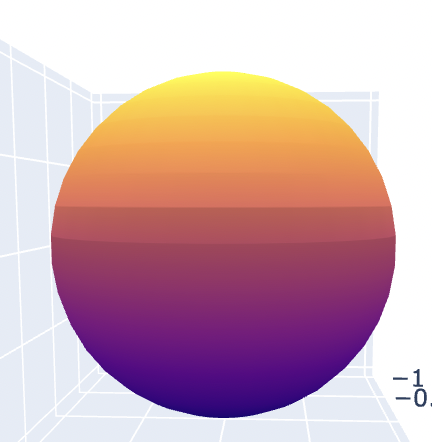
\includegraphics{images/sphere.png}


\section{Bayes Strategies}

So we have the tools we need to deal with decision making now. 

Given a set of strategies, we can construct some n-dimensional polyhedron(assuming there are n states of nature involved). There are two cases here: Either a set of admissible strategies exists, an indifference curve if you will, that is convex(not as a set but as a function) or flat to the origin on the sides of the surface closest to it - or the shape contains the origin, in which we can get arbitrarily close to an admissible point but no point will theoretically be admissible.  We will concern ourselves with the first case. It is important to note that there will always be some surface that contains the set of indifference points or admissible strategies for Mr. Nelson. 

In this case, how does Mr. Nelson differentiate between the 'indifference curve' formed by his admissible strategies? That's where the Bayes Strategy comes in. Given a prior belief about the states of nature, i.e that they occur with some probability, Mr. Nelson no longer has an indifference amongst his admissible strategies. In this case, the optimal solution is the point where the plane formed by the three probabilities on the states of nature is tangent to the convex closest surface of Mr. Nelson's set of strategies. 

Why is this a Bayes Strategy? Because where the plane defining our apriori belief of the states of nature (i.e if it will rain, rain heavily or be sunny) is tangent to the set of strategies is the point or set of points that minimizes the expected losses. 

\section{MinMax}
MinMax functions similarly to the Bayes strategy except, as the textbook illustrated with its example of Mr.Nelson's advice-giving friends - it is the pessimists solution. It is the strategy for which the maximum possible loss is the smallest of all maximum possible losses from each strategy. 
The way this is calculated in three dimensions is by defining a cube. The levels of $\theta_1$, $\theta_2$ and $\theta_3$ at which the cubes intersect the same convex/straight line surface we've discussed thus far in regards to the Bayes Strategies is the minmax solution. Why is this useful? It reduces the ceiling of expected loss. Applications can include investments, market inefficiencies, legal liability calculations - any scenario where it is important to make sure the worst case scenario is the least bad as can be. 

\section{A brief chat about computing in this chapter}

A lot of the treatment of analysis in this chapter focused on graphical methods. While I've tried my best to describe them here and graphed a few three dimensional objects in the 3Dplots jupyter notebook, my programming of 3D shapes needs some work. But the focus on computation for this chapter would be to replicate and create those kinds of surfaces to really help visualize what this kind of decision theory entails.  

\section{Mathematical ruminations}
What's been really interesting about following this chapter has been considering the implications in higher dimensions of these strategies. In generalizing what the book talked about and my own three dimensional foray into Mr. Nelson's strategies, this is what I've come up with: The convex set of strategies, by it's definition dictates that the admissible strategies form a n-1 dimensional surface in the region that the function that defines that surface has both a negative definite Jacobian and a negative definite Hessian. For a given polyhedron formed by strategies, identifying the Bayes strategy is then a case of fitting the closest such surface to the shape. This reeks of familiarity, of fitting some sort of smooth curve to spiky data and likely a lot of the optimization techniques and fitting approaches from MA679 will help solve this problem. Specifically, we can train some sort of cubic spline with an additional constraint of convexity or a support vector machine. 

\vspace{5mm} %5mm vertical space
An example of when I'd want to use these techniques:
If i have a portfolio of financial assets and want to minimize my loss, I'd create a polyhedron of losses from each strategy, build a confidence interval around the resulting polyhedron and fit an indifference curve to it. Then given my prior beliefs about the direction markets will head in, I can optimize strategy. If this sounds an awful lot like Markowitz portfolio theory but with extra steps, it sounds that way to me too, just with some rotation in space or reflections across axes. 

\end{document}
